\documentclass[../main/report.tex]{subfiles}
\begin{document}

\section{Troubleshooting and Workarounds}

During testing, it became apparent that there were two major issues that needed to be fixed with the PCB.
Firstly, the pin on the FPGA used for the clock was not one of the dedicated clock pins.
Secondly, the clock component had not been implemented according to spec.

\subsection*{FPGA clock pin problem}
An error with the pin connection between the FPGA and the clock was discovered during testing.
The FPGA demanded a special pin for the clock, but the PCB routed the clock to a regular GPIO pin.
After checking the PCB layout, a pin on the EBI bus was shown to be able to work as clock for the FPGA.

Since the clock is connected by jumpers to the FPGA, the pin on the EBI bus could be wired to the clock jumper on the FPGA, solving the problem.

\subsection*{Wrong implementation of the clock}

Due to a poor schematic in the clock component datasheet, the clock was wired incorrectly on the PCB, as illustrated in figure \ref{fig:pcb-clock}.

\begin{figure}[H]
    \centering
    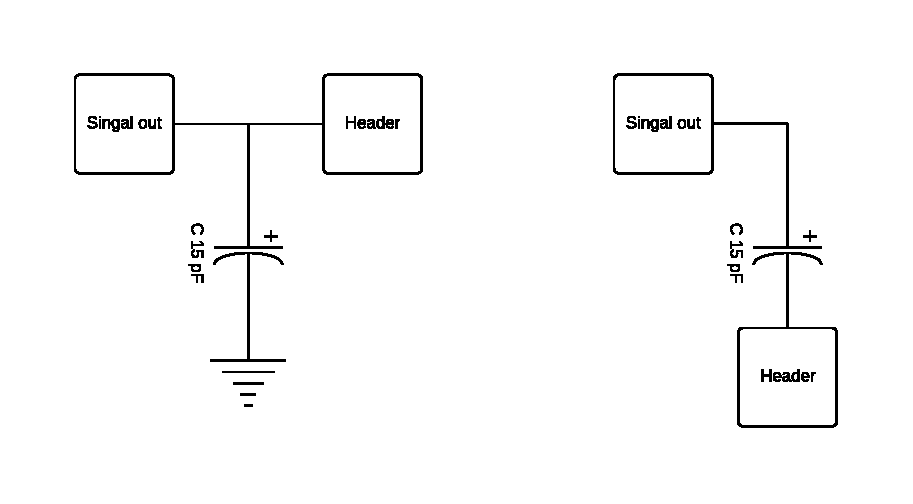
\includegraphics[width=0.8\textwidth]{../pcb/assets/pcb-clock.pdf}
    \label{fig:pcb-clock}
    \caption{On the left: How the clock from the FPGA should be connected.
             On the right: how it was connected on the PCB.}
\end{figure}

Because of this, the clock did not work.
This problem was solved by soldering together the pads of the SMD (surface mounted device\todo{move this definition earlier in the report}) capacitor to allow the clock signal to flow freely to the header pin.
A through-hole version of the removed capacitor was placed on one of the soldering pads and the other end grounded, see figure \ref{fig:pcb-clock-fix}.
This caused the circuit on the PCB to match up with the correct circuit from the data sheet.

\begin{figure}[H]
    \centering
    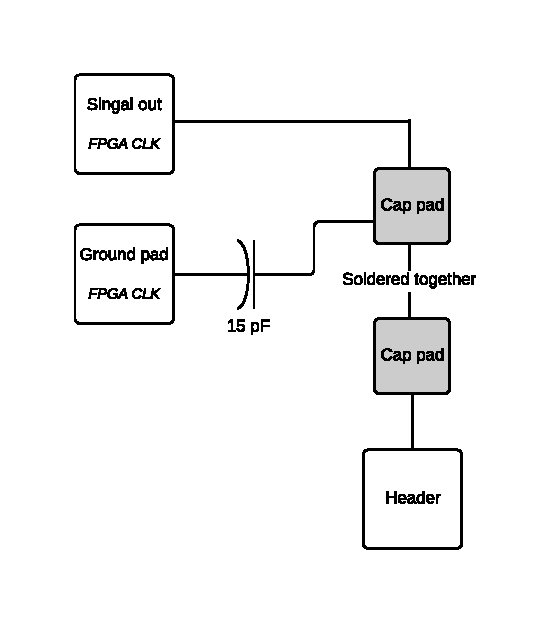
\includegraphics[width=0.7\textwidth]{../pcb/assets/pcb-clock-fix.pdf}
    \label{fig:pcb-clock-fix}
    \caption{How the FPGA clock fix was implemented.}
\end{figure}

\subsection*{Mismatch LDO}
During the testing phase, the LDO for the 1.2V did not output the correct voltage.
The 1.2V LDO is the same model as the 3.3V LDO, but has a different
footprint, see figure \ref{fig:ldo-footprints}.

It was assumed that both components had the same, which resulted in mismatch between the footprint and the component.
The solution was to place the LDO diagonally, \todo{insert the picture of the LDO?} and manually solder a wire to the correct solderpad on the PCB. 

\begin{figure}[H]
    \centering
    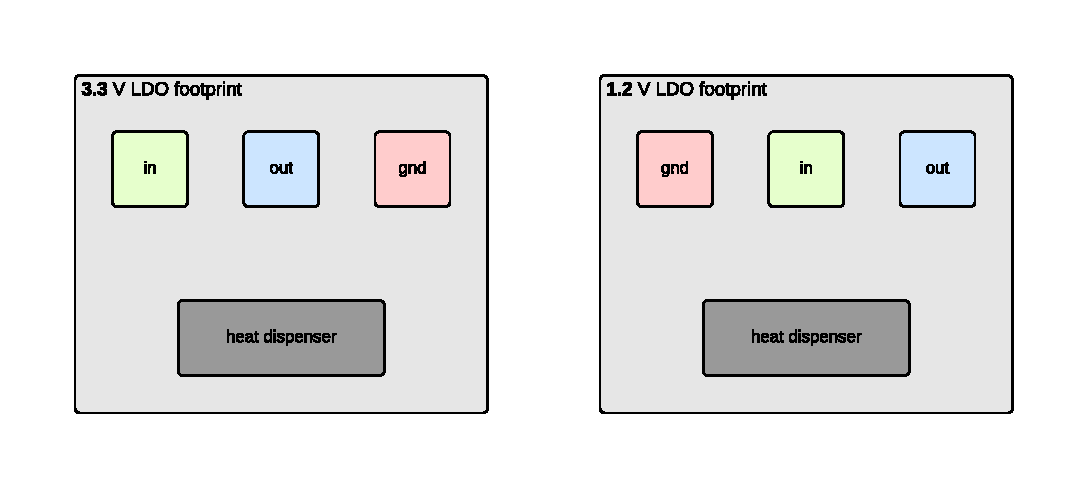
\includegraphics[width=\textwidth]{../pcb/assets/ldo-footprints.pdf}
    \label{fig:ldo-footprints}
    \caption{On the left: 3.3 V LDO footprint. On the right: 1.2 V LDO footprint.}
\end{figure}

\end{document}
